\subsection{Problem definition}

A 1D test example for groundwater flow and simultaneous heat transport in the aquifer is made. The aim of the numerical simulation with GeoSys/RockFlow is to determine if the consideration of varying density with temperature changes is possible. The following assumptions will be made:

\begin{tabular}{ll}
Aquifer: & homogeneous, saturated, stationary flow\\
Fluid flow: & incompressible fluid, non-isothermal.\\
\end{tabular}

\subsection{Model set-up of the 1~D numerical model}

For the 1-dimensional calculation the calculation area is simplified as a line of a length of $\unit[5.2]{m}$. The calculation model includes 25 elements and 26 nodes. The initial pressure in the whole area is $\unit[100]{kPa}$ and the initial temperature $\unit[300]{K}$. As boundary condition a constant pressure of $\unit[101]{kPa}$ is given at the left boundary and of $\unit[100]{kPa}$ at the right boundary. A constant temperature of $\unit[400]{K}$ is set at the left boundary. The used soil parameters are listed in Tab.~\ref{tab41}. The fluid density is decreasing with increasing temperature. The viscosity, capacity and conductivity of water are set to constant values. The fluid parameters also can be found in Tab.~\ref{tab41}.
\begin{table}[htbp]
\caption{\label{tab41}Used soil and fluid parameters.}
\begin{center}
\begin{tabular}{ll}
\toprule
parameter 			& value \\
\midrule
\multicolumn{2}{c}{\textit{soil parameters}}\\
porosity $\phi$   	& 0.01 \\	
permeability $K$   	& $\unit[1.0 \cdot 10^{-11}]{m^{2}}$ \\
density $\rho$     	& $\unit[2850]{kg \cdot m^{-3}}$ \\
%heat expansion    	& $\unit[1 \cdot 10^{-5}]{K^{-1}}$ \\
heat capacity $c_s$   	& $\unit[1000]{J \cdot kg^{-1} \cdot K^{-1}}$ \\
heat conductivity $\lambda_s$	& $\unit[3.2]{W \cdot m^{-1} \cdot K^{-1}}$ \\
\cmidrule{1-2}
\multicolumn{2}{c}{\textit{fluid parameters}}\\
initial density $\rho_0$ 	& $\unit[1000]{kg \cdot m^{-3}}$\\
viscosity $\eta$        	& $\unit[0.001]{N \cdot s \cdot m^{-2}}$ \\
heat capacity $c_f$    	& $\unit[4000]{J \cdot kg^{-1} \cdot K^{-1}}$ \\
heat conductivity $\lambda_f$	& $\unit[0.6]{W \cdot m^{-1} \cdot K^{-1}}$ \\
\bottomrule
\end{tabular}
\end{center}
\end{table}

\subsection{Validation method}

In order to find out whether the consideration of varying water density with temperature changes is possible, one simulation run is done with a constant density of $\unit[1000]{kg/m^{3}}$, which is the initial water density before heating, and one run with a constant density of $\unit[900]{kg/m^{3}}$, the density after the heating process. The temperature results for a heat transport with varying density have to be in between both temperature evolution curves.

\subsection{Results}

The curve for temperature evolution, which is shown in Fig.~\ref{figHT1} for the right boundary (node 26), shows the expected characteristics. Therefore it can be stated, that the consideration of temperature dependent fluid density is possible.
\begin{figure}[htbp]
\centering
\includegraphics[width=0.85\textwidth]{T/figures/figHT1.eps}
\caption{\label{figHT1}Temperature evolution with constant and variable fluid densities.}
\end{figure}

\begin{table}[H]
\caption{Benchmark deposit}
\begin{center}
\begin{tabular}{lll}
\toprule
Deposit & Version & Date \\
\midrule
$\backslash$HT\_var\_density\_1D & rf4.7.02 & March 2008\\
\bottomrule
\end{tabular}
\end{center}
\end{table}
%\clearpage


